\section{Beat Box}
Amb la melodia i l'harmonia, el ritme és un dels components més importants de la música. El mòdul ``Beat Box'' explora diverses maneres de crear i analitzar ritmes amb mètodes matemàtics.

\subsection{El Ritme de Fibonacci / Els nombres d'Hemachendra (Fibonacci) i els ritmes 2-1}

Rarament es s'anomena un concepte científic amb el nom de la persona que primer hi va tractar. Aquest és el cas dels famosos nombres de Fibonacci. Fibonacci va mencionar-los en un exercici de càlcul al seu llibre Liber Abaci publicat l'any 1202. De totes maneres, ja al voltant de l'any 1050, l'erudit indi Hemachendra ja havia estudiat aquests nombres en un context relacionat amb el ritme.

\begin{wrapfigure}{l}{0.4\textwidth}
\centering
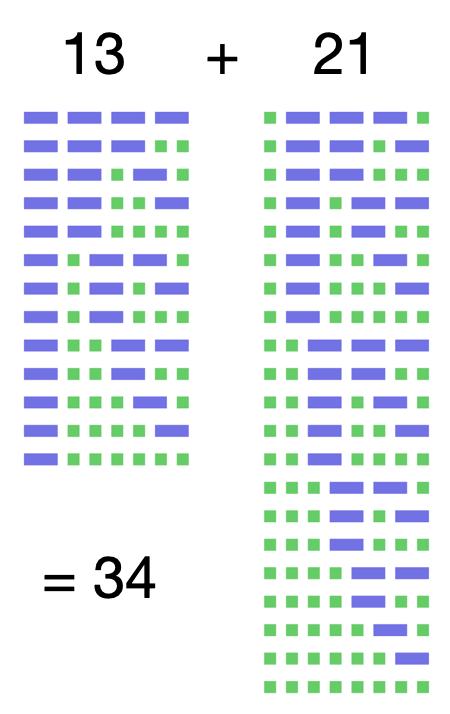
\includegraphics[width=0.4\textwidth]{BeatBox_1}
\caption*{Fibonacci rhythm}
\end{wrapfigure}

Imagina que vols omplir un ritme amb un nombre n de pulsacions amb patrons de longitud 1 o 2. Per exemple, un ritme de 8 pulsacions es podria omplir amb 1-1-1-1-1-1-1-1 o 2-2-2-2 o altres patrons més complicats, com ara 2-1-2-1-2 o 2-1-2-2-1. Quantes possibilitats hi ha? Aquest tipus de preguntes apareixen tant a la poesia quan parlem sobre versos i síl·labes, coma a la música quan parlem de ritmes fets amb blanques i negres. Resulta que el nombre de possibilitats és un nombre de Fibonacci (o, encara millor, d'Hemachendra). Un nombre de la seqüència:

1, 1, 2, 3, 5, 8, 13, 21, 34, 55, 89,144,...

On (després de començar amb 1, 1) cada nombre és la suma dels dos anteriors. De fet, hi ha exactament 34 maneres d'omplir un patró de 8 pulsacions amb uns i dosos.

\paragraph{La Música:}
Per evitar patrons repetitius a la música, a vegades és bo tenir en compte totes les possibilitats que satisfan cert requeriment. La qüestió d'omplir les pulsacions amb notes llargues i curtes, per exemple, té moltes aplicacions a l'art de tocar la Tabla. Aquí, sovint, les notes curtes i llargues no són literalment una nota sinó els patrons de tamborineig que omplen o bé una o bé dues pulsacions. Fent servir només dos patrons fixos, però essent flexible al nivell macro rítmic a l'hora de combinar-los  crea una coherència estilística aportant alhora riquesa.

\paragraph{Les Mates:}
Perquè els nombres de Fibonacci apareixen en aquest context? Anem a veure com podem reduir el problema d'omplir les 8 pulsacions a omplir-ne 6 o 7. Cada ritme de 8 pulsacions comença o bé amb una nota curta o una llarga.  Si comencem amb una nota curta hi ha tantes possibilitats d'omplir les posicions restants com n'hi haurien si haguéssim d'omplir només 7 pulsacions. Si, per altra banda, posem una nota llarga, existeixen les mateixes possibilitats per omplir la resta que hi haurien si n'haguéssim d'omplir 6. D'aquesta manera, el nombre de patrons de 8 pulsacions és igual a la suma del nombre de patrons de 7 pulsacions i de 6 pulsacions. Voilà! La successió de Fibonacci.

\paragraph{El Mòdul:} Aquest mòdul és bàsicament una Tabla rítmica automàtica basada en les observacions que hem fet abans. Com a curiositat, les mostres de so pel ritme ràpid es van extreure d'una xerrada del Manjul Bhargava, un matemàtic canadenc que ostenta una Medalla Fields, que va fer xerrades molt inspiradores sobre aquest tema, ja que ell mateix toca la Tabla.

\subsection{Aplaudiments  / La música d'aplaudiments de Steve Reich}
Vols un repte? Aquí el tens! Prova d'aplaudir al ritme d'una de les dues veus del mòdul d'aplaudiments. O, encara millor, prova amb algú altre a aplaudir alhora les dues veus. Per cada posició del punt verd el repte és diferent.

La peça que sents en aquest mòdul és un exemple impressionant de com una idea tan simple pot  crear patrons musicals tan complexos i interessants. Inspirat en els aplaudiments del Flamenc, Steve Reich va compondre aquesta petita peça. Consisteix en un patró d'aplaudiments de 12 pulsacions:


\begin{figure}[h]
\centering
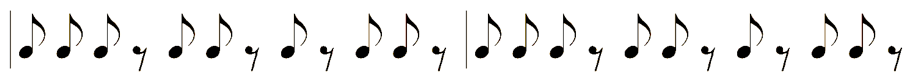
\includegraphics[width=0.9\textwidth]{BeatBox_2}
\end{figure}

3 aplaudiments - pausa - 2 aplaudiments - pausa - 1 aplaudiment - pausa - 2 aplaudiments  - pausa ... i repeteix

La complexitat s'aconsegueix tocant exactament el mateix ritme amb dues o més persones, però desplaçant el començament n pulsacions, on n pot anar del 0 fins a l'11. D'aquesta manera hi ha fins a 12 possibles resultats. Pots fer-los tots amb algú altre?

\begin{wrapfigure}{l}{0.35\textwidth}
\centering
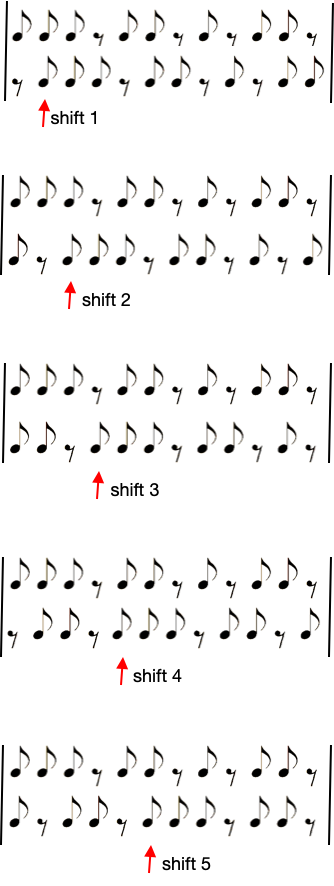
\includegraphics[width=0.35\textwidth]{BeatBox_3}
\end{wrapfigure}

\paragraph{La Música:}
Una Música Mínima ( bàsicament composta per Steve Reich) intenta crear música interessant amb progressions minimalistes de la partitura. Desplaçar un patró rítmic només una pulsació es pot considerar com un element típic de progressió de la Música Mínima. De fet, la peça d'aplaudiments necessita una enorme concentració des del moment en què les dues persones comencen a tocar juntes. Per això, tot i ser mínima, no és en cap cas fàcil.

\paragraph{Les Mates:}
Quants patrons rítmics són adients per crear una peça com la música d'aplaudiments? Quedem-nos amb les seqüències d'una i dues pulsacions. Per començar, hi ha un total de $2^{12} = 4096$ possibilitats de tenir o bé pausa o bé aplaudiment a cada pulsació.

Podríem voler que cada patró en sí mateix no tingués repeticions, ja que causaria música idèntica cada desplaçament. Això descarta 76 d'aquests patrons. Dels 4020 restants només necessitem una versió desplaçada de cada un. Això ens divideix el nombre total per 12 i ens deixa amb només 335 patrons.

La majoría sonarien força avorrits, ja que hi hauria o bé massa o bé massa pocs aplaudiments. Si ho restringim a un mínim de 4 aplaudiments i un màxim de 8, ens deixa amb 287 possibilitats. Si encara ho volem restringir més, podem exigir que no hi hagi pauses consecutives. Això ens deixa amb només 11 patrons (mostrats a sota). El patró que va escollir Steve Reich (marcat en vermell) és un dels dos únics patrons que no repeteix el nombre d'aplaudiments entre dues pauses.

\begin{figure}[h]
\centering
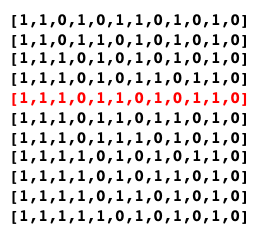
\includegraphics[width=0.4\textwidth]{BeatBox_4}
\end{figure}

%
%[1,1,0,1,0,1,1,0,1,0,1,0]
%[1,1,0,1,1,0,1,0,1,0,1,0]
%[1,1,1,0,1,0,1,0,1,0,1,0]
%[1,1,1,0,1,0,1,1,0,1,1,0]
%[1,1,1,0,1,1,0,1,0,1,1,0]
%[1,1,1,0,1,1,0,1,1,0,1,0]
%[1,1,1,0,1,1,1,0,1,0,1,0]
%[1,1,1,1,0,1,0,1,0,1,1,0]
%[1,1,1,1,0,1,0,1,1,0,1,0]
%[1,1,1,1,0,1,1,0,1,0,1,0]
%[1,1,1,1,1,0,1,0,1,0,1,0]
%

\paragraph{El Mòdul:}
Prova d'aplaudir! Comença a poc a poc i vés incrementant la velocitat. Selecciona diferents desplaçaments movent el punt verd al cercle.


\subsection{Seqüenciador}
Has entrat mai a la sala d'impressió d'algun gran diari?
On les màquines giren una vegada i una altra i creen un patró de so amb cada rotació. O una màquina de cosir? Sempre que un procés mecànic produeix un patró repetitiu el nostre cervell intenta descobrir l'estructura que s'hi amaga. Formant ritme. Formant música. La màquina de ritmes de la nostra exposició és un seqüenciador que et permet experimentar amb patrons cíclics. Juga-hi i explora!

\paragraph{El Mòdul:}
Potser pot anar bé una mica d'informació d'ús. Imagina les quatre rodes grans com tocadiscs equipats amb barres. Sempre que les barres toquen un instrument aquests creen un so. Els instruments es representen amb els cinc punts de colors de l'àrea central. Pots moure'ls lliurement. Si els colpeja alguna cosa produiran un so. Quin instrument representa cada punt es pot triar amb els botons lliscants de colors a la dreta. Com més a l'exterior de la roda es col·loqui un instrument, més fort sonarà.

Quan la màquina està en repòs, el nombre de barres de cada disc es pot canviar movent els botons lliscants. Amb això, es poden crear patrons de repetició molt irregulars però, tot i això, cíclics. Per exemple, pots posar un dels discs a 8 barres per gir, un altre a 11 i els altres dos a 15. Això pot sonar estrany, però pot ser molt rítmic. Com a curiositat, les cultures africanes estan molt més acostumades als ritmes irregulars que les cultures occidentals.

\begin{figure}[h]
\centering
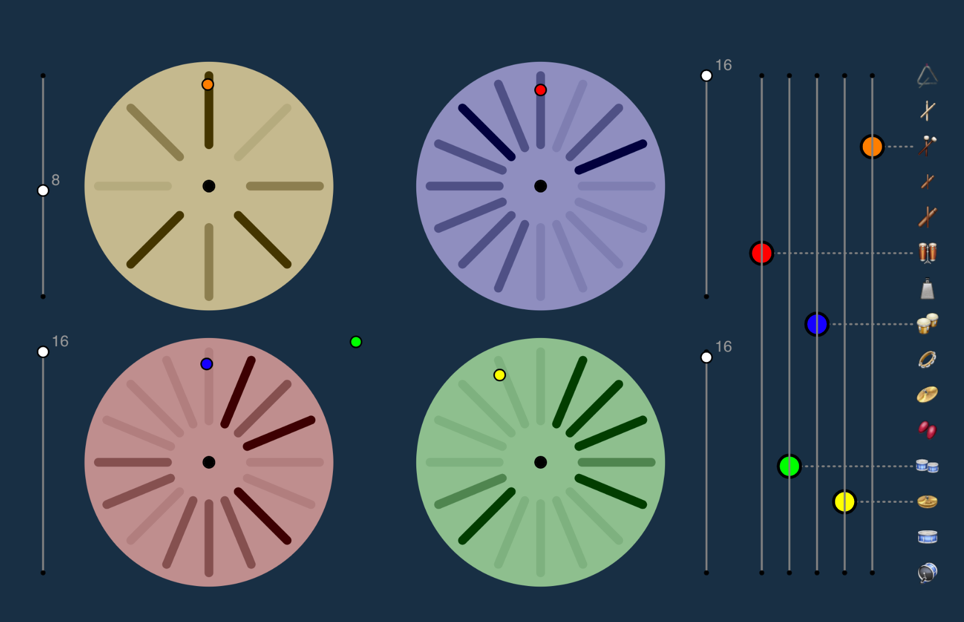
\includegraphics[width=0.9\textwidth]{BeatBox_5}
\end{figure}

En l'estat de repòs també pots clicar a les barres per canviar-ne l'estat entre els tres disponibles: fort, mitjà, apagat. Amb això pots crear una gran varietat de ritmes tan coneguts com totalment nous!

\subsection{Ritmes de n sobre m}
Estem molt acostumats a aplaudir ritmes regulars simples com un pas doble 1-2-1-2-1-2 o un vals en compàs de 3 1-2-3-1-2-3. Això és, potser, un dels primers exercicis que es fan quan es comença amb un instrument de percussió. Però les coses es tornen realment complicades quan volem aplaudir dos ritmes alhora. Combinar un ritme regular amb n pulsacions en un compàs amb un altre ritme amb m pulsacions per compàs alhora s'anomena ritme de n sobre m. La ràtio de velocitat entre els dos ritmes és n/m. La fotografia de sota il·lustra ritmes de 2 sobre 3. A cada compàs, la veu de dalt té dues notes perfectament distribuïdes i la de sota en té tres.

\paragraph{Les Mates:}
Potser la manera més fàcil d'aprendre ritmes n sobre m és barrejar-los en un marc de tics consonants prou bo per posar-hi els dos ritmes. Matemàticament això demana el mínim comú múltiple dels dos nombres n i m. Així un ritme de 2 sobre 3 es pot col·locar en un ritme regular de 6 tics, un 3 sobre 4 en 12 tics i un 7 sobre 5 en un ritme de 35. Si comptem els tics des de 0, el ritme de m pulsacions es tocarà als múltiples de n i el de n es tocarà als múltiples de m.

\begin{figure}[h]
\centering
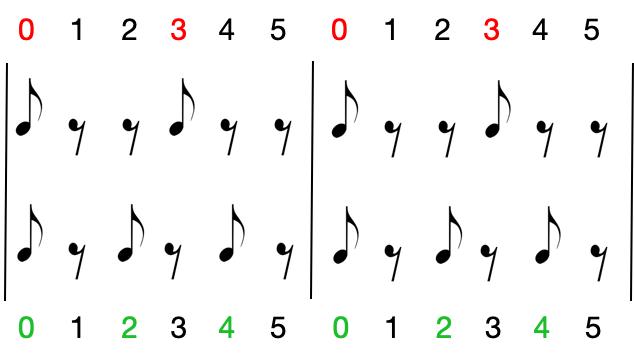
\includegraphics[width=0.7\textwidth]{BeatBox_6}
\end{figure}

\paragraph{La Música:}Tocar el ritme de n sobre m de la manera mencionada és una molt bona manera d'aprendre'n. De totes maneres té un gran desavantatge. No ``sents'' el ritme com si estigués fet per dos de diferents i més simples.

Aquí teniu un ``pro tip'' per aprendre aquests ritmes. Primer aprèn a aplaudir-los amb les dues mans fent servir el mètode mencionat (trigaràs una mica). Quan et sentis segur aplaudint aquests ritmes, fes-los i intenta ``separar la teva ment'' i concentrar-te en només una mà i el que fa. Després canvia a l'altra mà. En algun moment seràs capaç de sentir els dos ritmes de forma independent i alhora a la teva ment.

\begin{figure}[h]
\centering
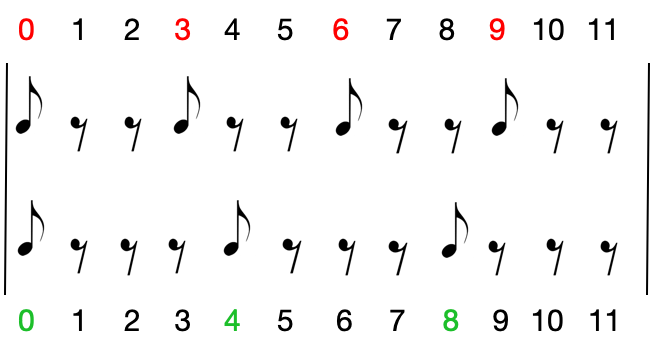
\includegraphics[width=0.7\textwidth]{BeatBox_7}
\end{figure}

\paragraph{El Mòdul:} Aquest mòdul busca que aplaudeixis amb ell. Pots escoltar i experimentar ritmes n sobre m i també pots intentar aplaudir-los. Pot ser que requereixi una mica de pràctica, però un cop ho tinguis és una cosa que mai podràs oblidar.

\subsection{Ritmes de quadrícula}
Pots sentir el ritme d'un dibuix ornamental? Has corregut mai amb una maleta de rodes sobre un paviment regular per agafar el tren o un avió? Has sentit el so que feia la maleta amb el paviment? De fet, ja amb els patrons més simples (com una quadrícula), si hi movem un punt per sobre a velocitat constant, podem obtenir ritmes prou interessants. Si associes diferents veus a les línies horitzontals i verticals de la quadrícula quan mous el punt cap a qualsevol direcció amb velocitat constant crea un patró rítmic únic per cada veu. De totes maneres, els patrons tenen diferents velocitats i estan desplaçades en fase, deixant un munt d'espai per l'experiència musical.

\paragraph{La Música:}
Obtenir inspiració per crear patrons musicals interessants és una part molt important de la feina dels músics. Aquestes inspiracions poden venir de moltes fonts diferents.

Recomanem molt escoltar el vídeo ``Stoiber on Drums'' a YouTube en què un percussionista actua mentre
l'Edmund Stoibers parla sobre la connexió amb tren d'alta velocitat des del centre de Munich fins a l'aeroport intentant tocar un instrument cada vegada que hi ha una síl·laba a la xerrada.

\begin{figure}[h]
\centering
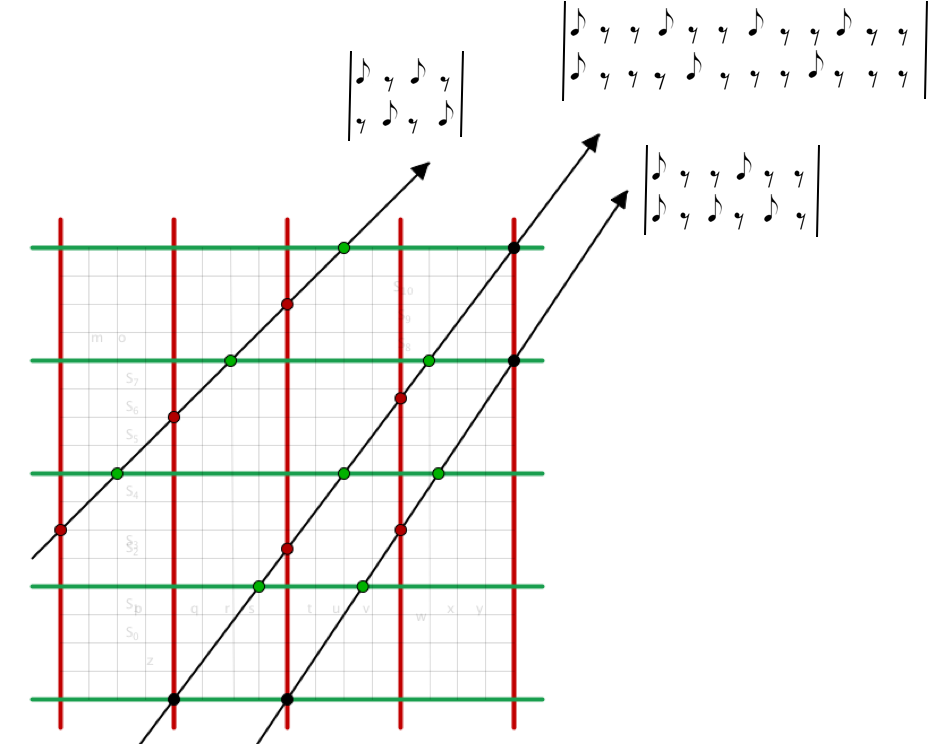
\includegraphics[width=0.7\textwidth]{BeatBox_8}
\end{figure}

\paragraph{Les Mates:} La quadrícula crea un espai de dos patrons regulars. En aquest context, excepte la regularitat, tota la resta és lliure per a cada patró: les dues velocitats i la fase entre ells. Els exemples a la figura en mostren alguns casos, entre ells un ritme 2 sobre 3 i un 3 sobre 4. Si el pendent de la línia és irracional (no és una fracció) llavors el patró rítmic generat no es repetirà mai.

\paragraph{El mòdul:}
Ajustant el pendent del moviment pots experimentar totes les possibilitats que es fan accessibles amb aquesta aproximació a la generació de ritmes. També pots ajustar la direcció del moviment de la quadrícula. Prémer un dels botons de sincronització posa la graella a la posició indicada respecte del punt de mesura. Això et proporciona una mica més de control sobre el ritme.

\subsection{Ritmes d'Euclides / Ritmes de pas de línia}
Com es distribueixen 3 cops de tambor en un compàs de 8 pulsacions? I quina relació té amb les pantalles d'ordinador de baixa resolució? Aquí apareix una connexió curiosa. Imagina que vols dibuixar una línia amb pendent 3/8 en una quadrícula de baixa resolució amb una línia pixelada. La imatge de sota mostra la línia vista com una seqüència de píxels destacats. Els passos en aquesta imatge formen un patró regular i rítmic. La pendent de 3/8 implica que per cada 8 unitats que et moguis cap a la dreta te n'has de moure 3 cap amunt. Per això el patró es repeteix cada 8 passos. Si toquessis el tambor cada vegada que et mous una unitat cap amunt, tindries un patró de 3 cops distribuits en 8 pulsacions.

\begin{figure}[h]
\centering
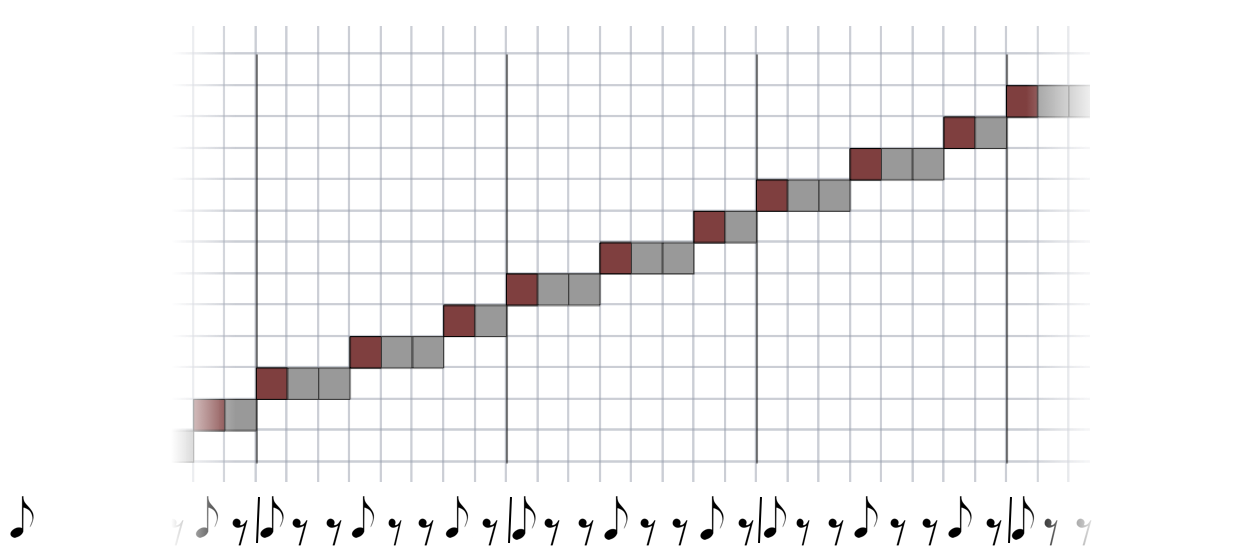
\includegraphics[width=0.7\textwidth]{BeatBox_9}
\end{figure}

\paragraph{Les Mates:}
Aquest mètode de generació de ritmes té una propietat remarcable. Distribueix els 3 cops de la manera més equitativa possible entre les 8 pulsacions. La raó d'això és que el dibuix pixelat de la línia l'aproxima tan bé com pot. Una altra manera de pensar en aquest mètode de generació és considerant un triangle de costats iguals i després triar punts d'un octàgon amb el mateix centre que estiguin el més a prop possible dels costats del triangle. Clarament aquest mètode es pot generalitzar a qualsevol nombre de cops i pulsacions.

\paragraph{La Música:} La distribució igual indicada en aquest mètode crea ritmes molt interessants. De fet, es poden trobar en un munt de cultures i estils. Des del folklore balcànic fins al Take Five de Dave Brubeck, passant pels ritmes  llatinoamericans i japonesos.

\paragraph{El Mòdul:} En aquest mòdul pots crear els dos ritmes mencionats en paral·lel i variar els números que generen els ritmes. És una gran eina per crear i dur a terme patrons rítmics elaborats.

\begin{figure}[h]
\centering
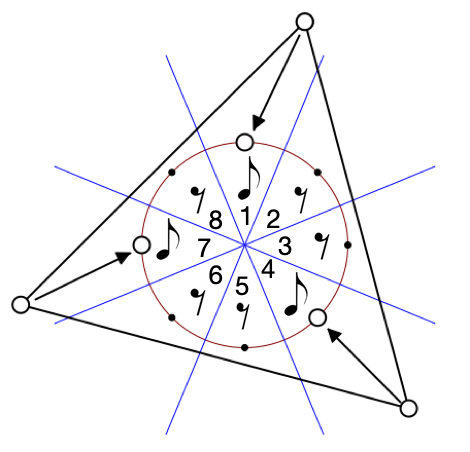
\includegraphics[width=0.4\textwidth]{BeatBox_10}
\end{figure}

\vfill

Autor del mòdul: Jürgen Richter-Gebert, Technical University of Munich
Motor de So: Patrick Wilson i Aaron Montag / basat en CindyJS.org
Text: Jürgen Richter-Gebert (TU Munich)
